\documentclass[11pt]{article}

\usepackage{sectsty}
\usepackage{graphicx}

% Margins
\topmargin=-0.45in
\evensidemargin=0in
\oddsidemargin=0in
\textwidth=6.5in
\textheight=9.0in
\headsep=0.25in

\title{\textbf{Dokumentation zu:\\DRL-Aufgabenblatt "Der K-armige Bandit"}}
\author{ Max Mustermann, Domenic Scholz}
\date{\today}

\begin{document}
\maketitle	
\pagebreak

%--Paper--

\section*{Aufgabe 1}
\subsection*{Aufgabe 1.1}
\subsubsection*{a)}
Abbildung \ref{img:1_1a} zeigt die initiale Auswertung des Banditenproblems. Um eine Mittelung der Ergebnisse zu erhalten, wurde das Experiment über zehn Durchläufe gemittelt. Die Parameter der Normalverteilungen der vier arme sind in Tabelle \ref{table:dist_1_1a} dargestellt.
\begin{table}[h]
    \centering
    \begin{tabular}{|c|c|c|}
        \hline
        Arm & Erwartungswert & Standardabweichung \\
        \hline
        1 & 2.62 & 2.78\\
        \hline
        2 & 1.35 & 0.93 \\
        \hline
        3 & 4.62 & 2.19\\
        \hline
        4 & 3.31 & 1.28\\
        \hline
    \end{tabular}
    \caption{Normalverteilungen der vier Arme Aufgabe 1.1 a)}
    \label{table:dist_1_1a}
\end{table}
\begin{figure}[h]
    \centering
    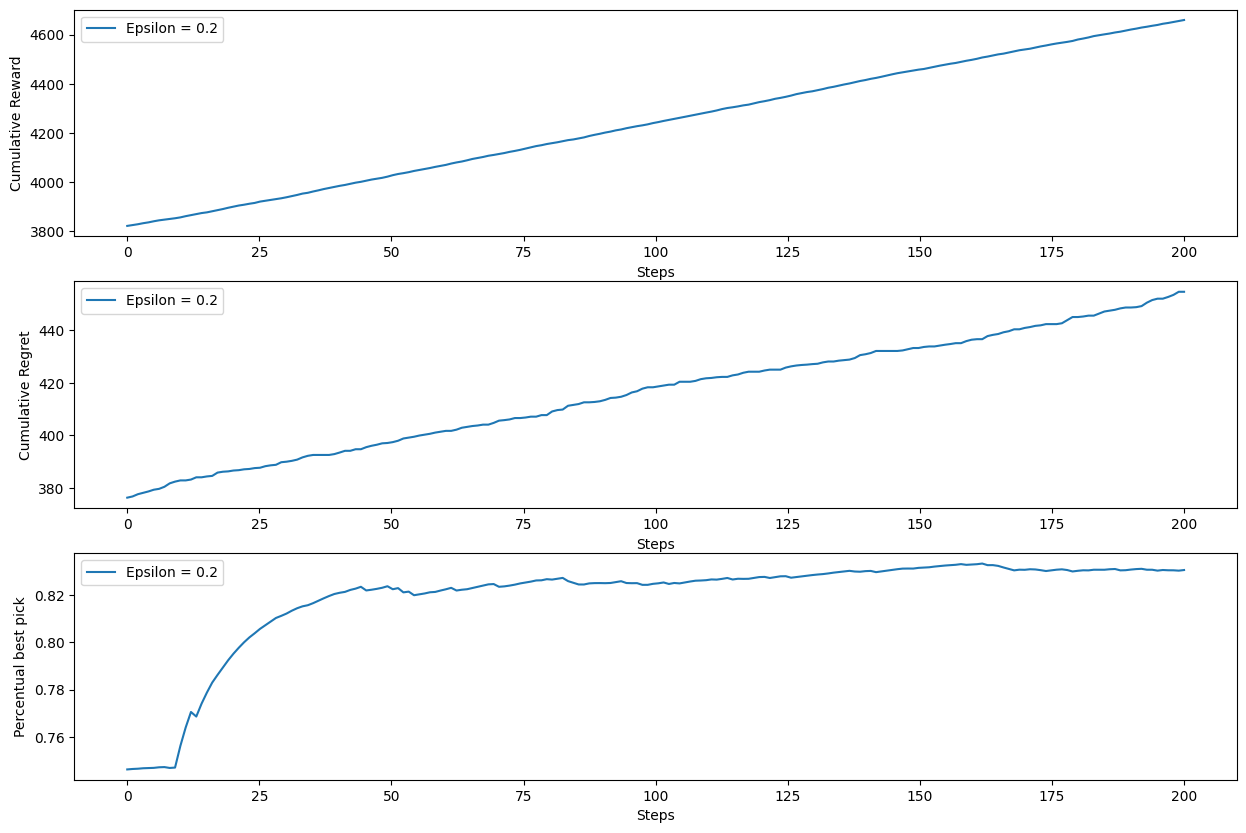
\includegraphics[width=\textwidth]{img/1_1a.png}
    \caption{Initiale Auswertung Banditenproblem}
    \label{img:1_1a}
\end{figure}
Die erste Auswahl des Arms erfolgt zufällig, alle darauffolgenden Auswahlen orientieren sich an der $\epsilon$-greedy Methode. Da hier mit einem $\epsilon$-Wert von $20\%$ gearbeitet wird, kann der Anteil der Fälle, in denen der beste Arm gewählt wird, $1-\epsilon = 80\%$ im Mittel nicht überschreiten. Dies ist in der untersten Grafik in Abbildung \ref{img:1_1a} dargestellt. Außerdem führt dies dazu, dass der kumulierte Regret über den Verlauf der Durchführung des Experiments nicht unbegrenzt lange auf dem gleichen Wert stagnieren kann. Da in $20\%$ der Fälle ein zufälliger anderer Arm gewählt wird, wird die Differenz der Erwartungswerte zum bisher gesammelten Regret addiert, sodass dieser steigt.
Dass der Verlauf des kumulierten Reward einer Gerade ähnelt, liegt daran, dass alle Erwartungswerte ähnlich sind und sich der Reward daher auch bei der Wahl des nicht optimalen Arms um einen nahezu gleichbleibenden Wert ändert. Zudem überwiegt der optimale Arm mit $80\%$ der Züge, sodass der geringere Reward durch die nicht optimalen Arme nur wenig ins Gewicht fällt. 
\subsubsection*{b)}
Abbildung \ref{img:1_1b} zeigt das Verhalten des Algorithmus bei verschiedenen $\epsilon$-Werten. Die zugrundeliegenden Normalverteilungen sind auch hier die aus Tabelle \ref{table:dist_1_1a}, außerdem wurde das Experiment für jeden $\epsilon$-Wert auch hier zehn Mal durchgeführt, um Mittelwerte zu erhalten. Es lassen sich zwei markante Dinge erkennen: Der Endwert der relativen Häufigkeit des optimalen Arms und die Dauer bis zum Erreichen des Endwertes. Kleinere $\epsilon$-Werte erlauben ein häufigeres Auswählen des besten Arms, das heißt, dass der Endwert der relativen Häufigkeit höher ist (siehe Grafik drei in Abbildung \ref{img:1_1b}). Da dies jedoch auch bedeutet, dass der Exploration-Anteil geringer ist, kann es unter Umständen länger dauern, bis das optimale Ergebnis gefunden wird, auch das lässt sich Grafik drei in Abbildung \ref{img:1_1b} entnehmen. Die Durchläufe, in denen der Exploration-ANteil $10\%$ bzw. $20\%$ beträgt, finden schneller das optimale Ergebnis als der Durchlauf mit nur $1\%$ Exploration-Anteil. 
\begin{figure}[h]
    \centering
    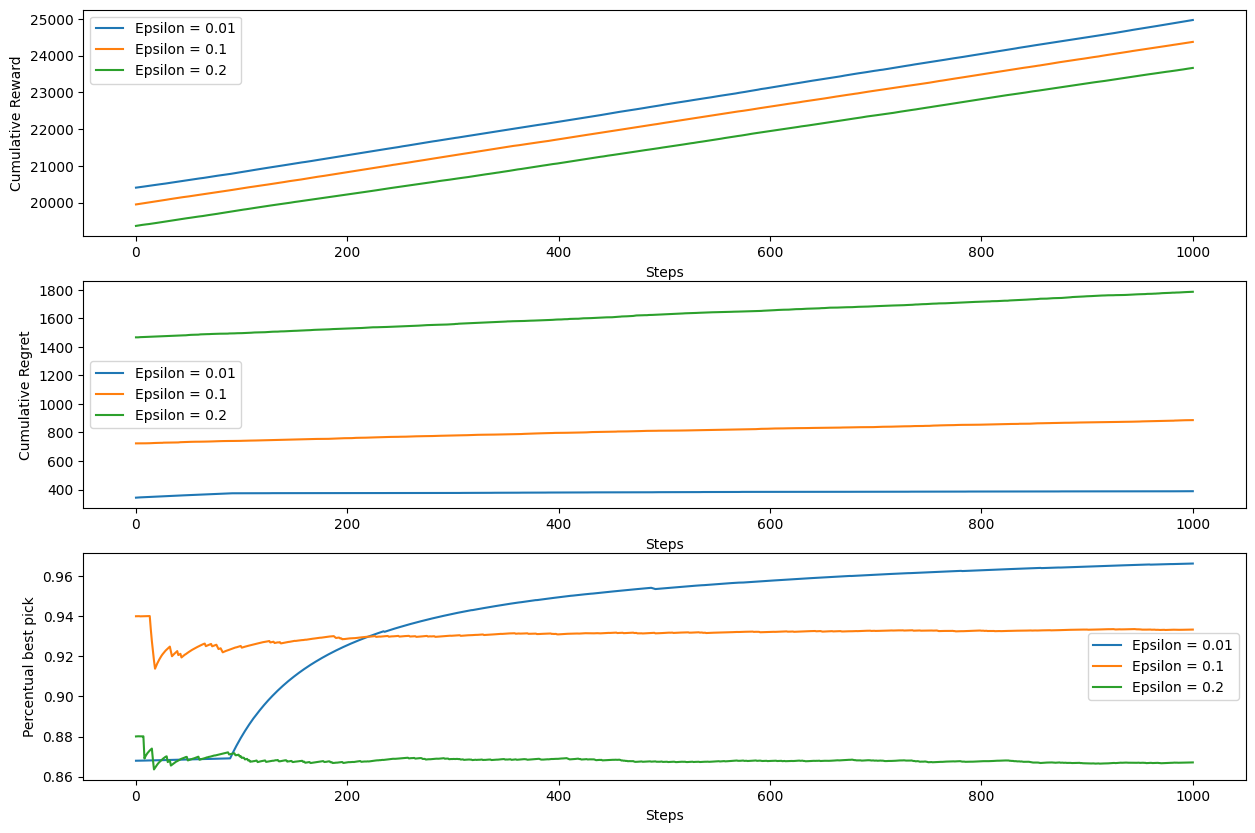
\includegraphics[width=\textwidth]{img/1_1b.png}
    \caption{Banditenproblem mit verschiedenen $\epsilon$-Werten}
    \label{img:1_1b}
\end{figure}
\subsubsection*{c)}
\subsubsection*{d)}
\subsection*{Aufgabe 1.2}
\subsubsection*{a)}
\subsubsection*{b)}
\subsubsection*{c)}
\subsubsection*{d)}

%--/Paper--

\end{document}